To evaluate the quality of our features, different architectures were implemented to compare how accurately they predict comment volume.
All seven architectural models use single or related features as input and generate a binary classification output using sigmoid as the activation function. 
Each model has an identifier which will be used as a reference within the further text.

\subsection{Architectures}

\paragraph{Model 1} 
Takes the article headline as input.
The headline length is normalized before embedding the words using an embedding layer which is initialized with pretrained glove embeddings \cite{pennington2014glove}.
The model uses a dense and a batch normalization layer as the hidden layers.

\paragraph{Model 2}
Takes the article headline as input which is than embedded as in \textit{Model 1}. 
A convolutional layer with kernel sizes one, three, and five is used instead of a dense layer as well as a pooling layer as proposed by Kim \cite{kim2014convolutional}.

\paragraph{Model 3} 
Takes the first $50$ words of the article text which are embedded the same way as in \textit{Model 1} and \textit{2}. However, the input is processed through an LSTM layer outputting its last cell state.

\paragraph{Model 4} 
Takes the article category as input.
The category reference gets embedded using an embedding layer and is processed through both a dense and a batch normalization layer.

\paragraph{Model 5} 
Takes temporal features of the article's publication date as input.
The features are minute, hour, day of the week, and day of the year.
They get processed the same way as in \textit{Model 4}.

\paragraph{Model 6} 
Takes the word counts from the headline and the article.
The logarithm is calculated for both of them and is used to create exponential sized bins for different lengths.
Each logarithm gets embedded and processed as in \textit{Model 5} and \textit{6}.

\paragraph{Model 7} 
Takes the competitive score as defined in \autoref{eq:competitive_score} and processes it through a dense layer as well as a batch normalization layer.

\subsection{Training}
The GACC was divided into training, validation, and test sets using a $0.70/0.15/0.15$  distribution with respect to the time of publication.

Due to the strongly imbalanced class sizes of the training set, we use class weights to penalise our models in case of a wrong classification.
During the training, they influence the weighting of the loss indirectly proportional to the class size of a giving training sample.

\subsection{Combined Architectures}
We combined several models to explore how using multiple features simultaneously would impact our results.
These combined models share the classification layers but not the hidden layers.
Specific models were only combined if they performed adequately and if their results had some correlation.
Combining these two metrics, we had a larger set of models we were able to choose from.
The correlations between each model pair are shown in Figure \ref{fig:correlation_matrix}. 

\begin{figure}[h]
	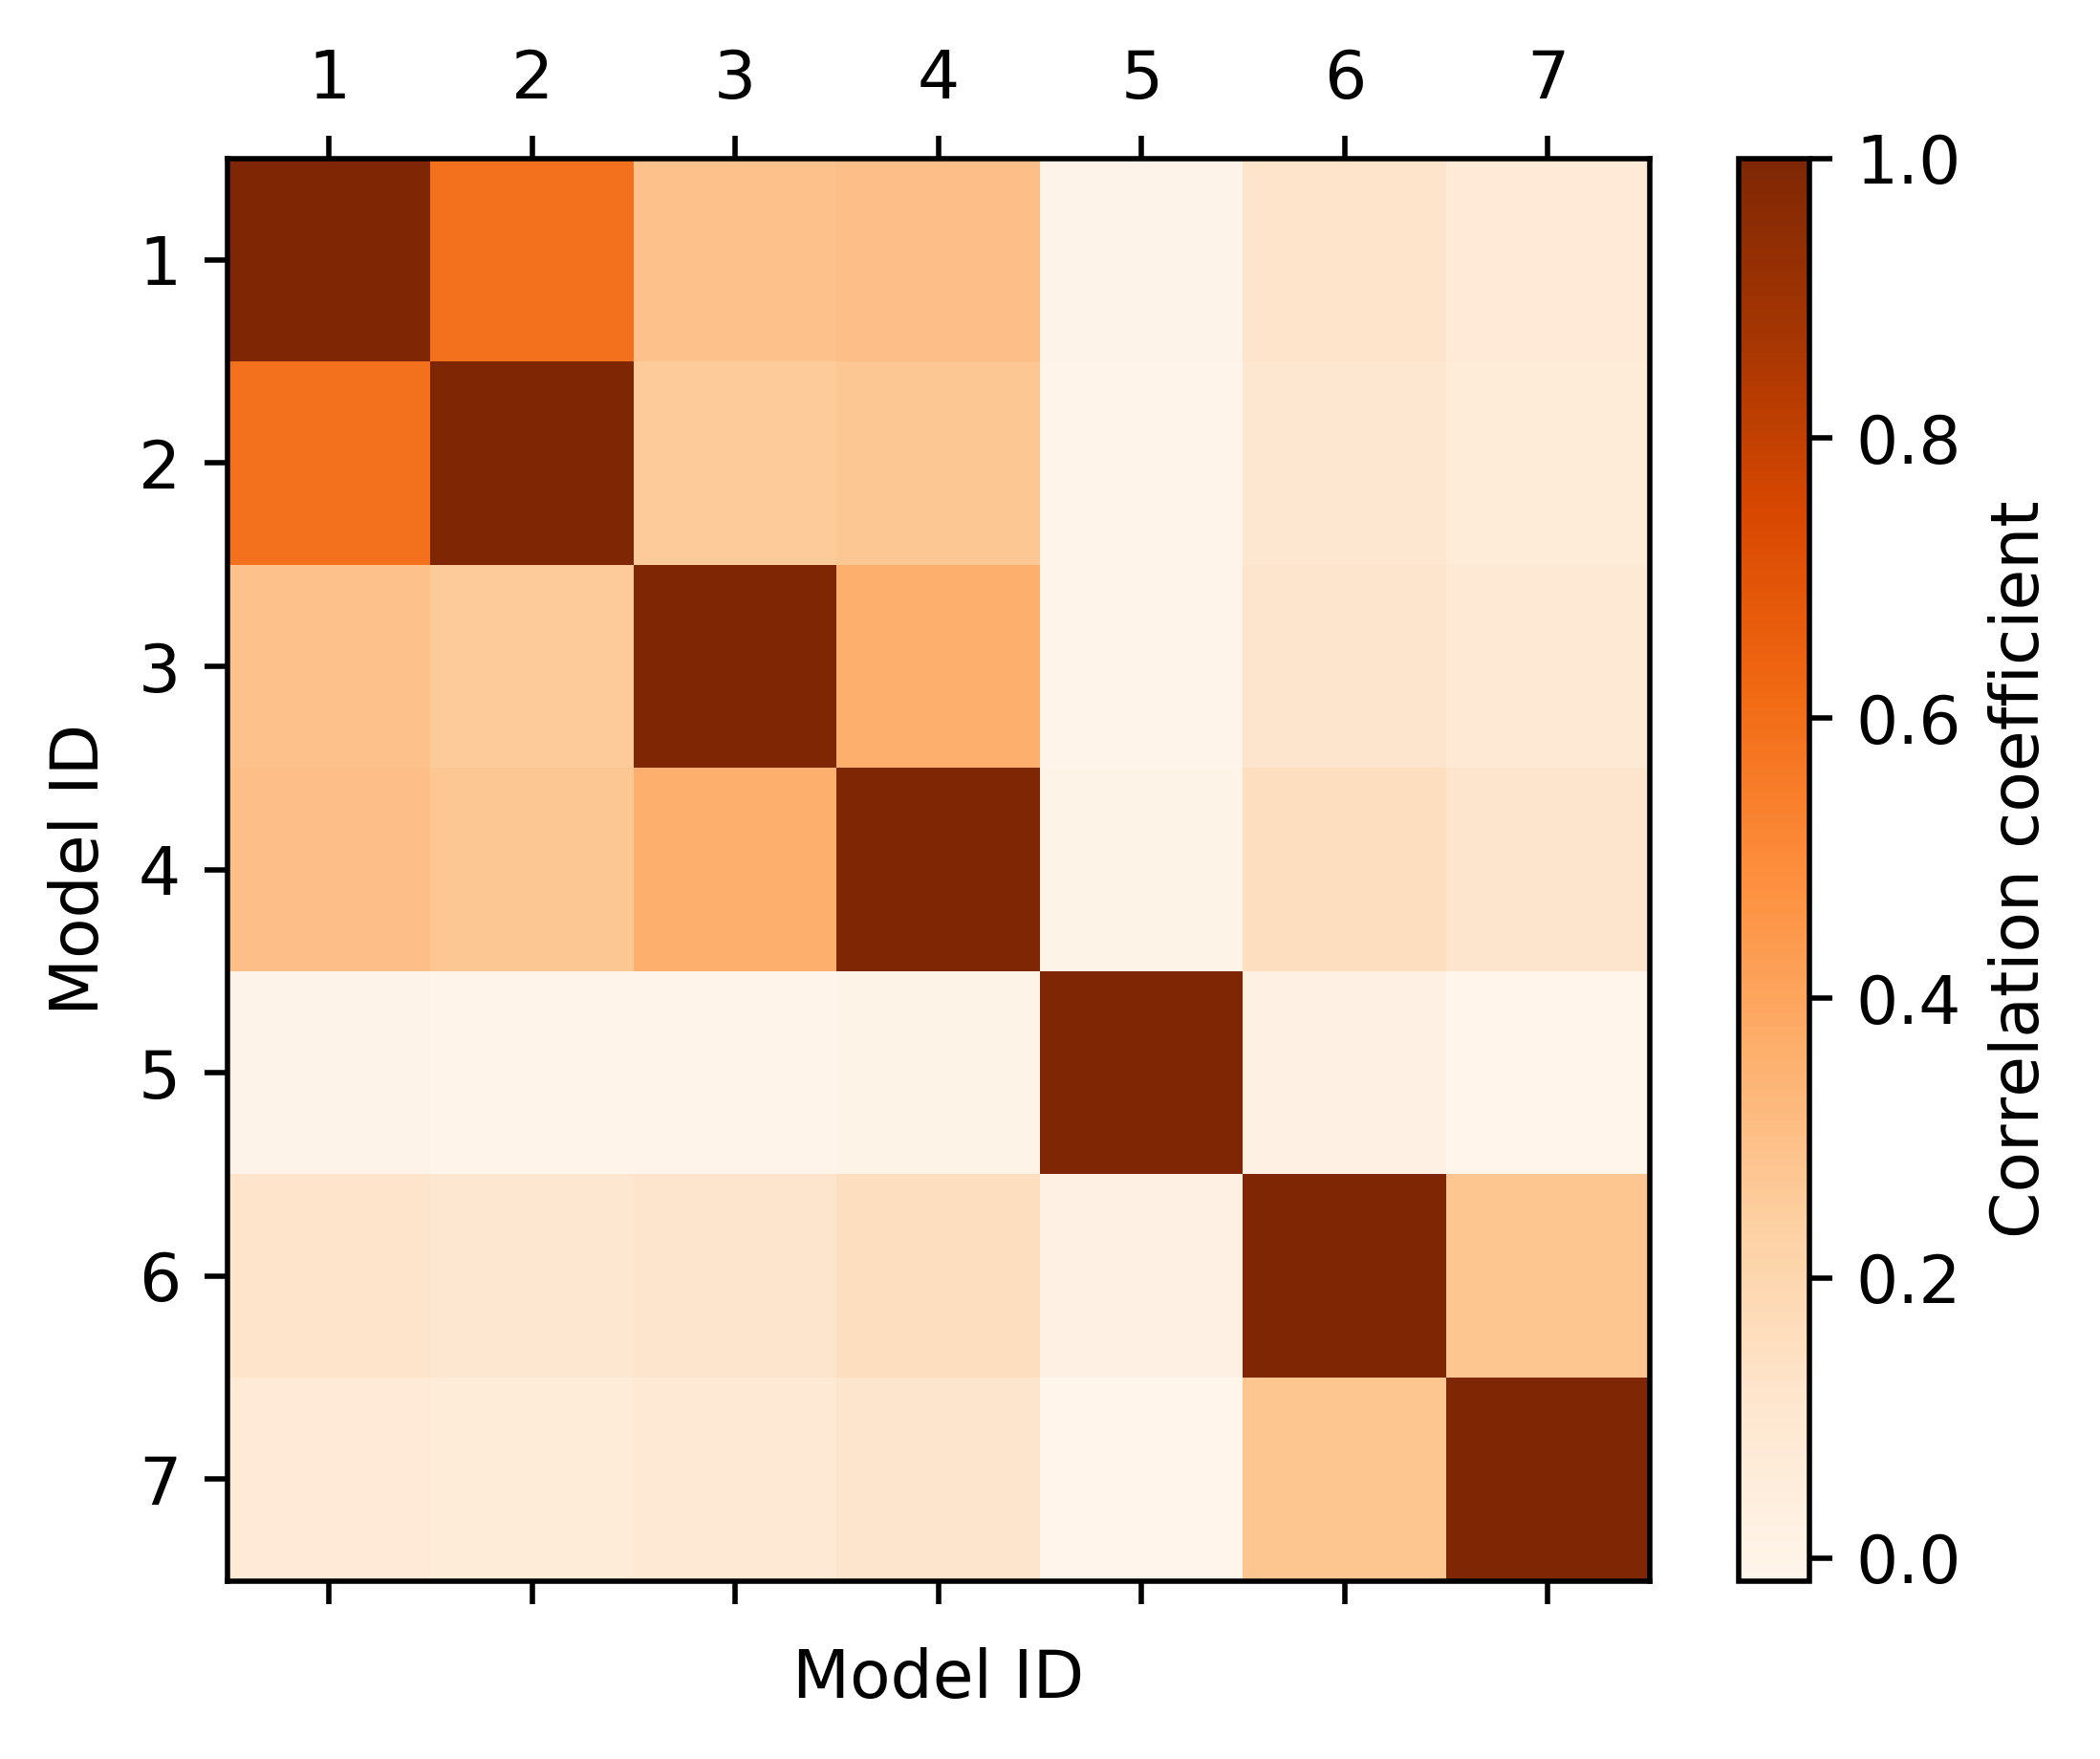
\includegraphics[width=0.3\textwidth]{fig/correlations.png}
	\caption{\textmd{Correlation matrix of our models using the test data set.}}
	\label{fig:correlation_matrix}
\end{figure}
